
\begin{figure}[H]
    Mezi uzly \(V_{CC}\) a \(GND\) je umístěn napěťový zdroj s napětím \(V_{CC} = 1.8 [V]\), pro zjednodušení jen není uveden ve schematu, což bude platit i u dalších zapojení.

    \vspace{8mm}
    \begin{minipage}{0.5\textwidth}
        \begin{circuitikz}[scale=1, transform shape] 
            \draw
              % MOSFET transistor with labels for drain (D), gate (G), source (S), and bulk (B)
              (0,0) node[nmos, bulk] (mos) {}
              (mos.drain) node[left] {M1}
            
              % Gate voltage source VGS
              (mos.gate) to[short, -] ++(-2,0) to[voltage source, l^=$V_{GS}$] ++(0,-1.5) node[ground] {}
              
              % Drain voltage source VDS (vertical)
              (mos.drain) to[short, -] ++(0,1) -- ++(2,0) -- ++(0,-1) to[voltage source, l^=$V_{DS} $] ++(0,-2) -- (2,-1.5) node[ground] {}
              
              % Source connected to ground, aligned with VGS ground
              (mos.source) to[short, -] (0,-1.5) node[ground] {}
              
              % Bulk (body) connection to ground
              (mos.bulk) to[short, -] (0.5, 0) -- ++(0,-1) -- ++(-0.5,0)  node[circle,fill,inner sep=1pt] (myNode) {}
            ;
        \end{circuitikz}

        \vspace{5mm}
        \centering{(NMOS)}
    \end{minipage}
    \hfill
    \begin{minipage}{0.5\textwidth}
        \begin{circuitikz}[scale=1, transform shape] 
            \draw
              % MOSFET transistor with labels for drain (D), gate (G), source (S), and bulk (B)
              (0,0) node[pmos, bulk] (mos) {}
              (mos.drain) node[left] {M1}
            
              % Gate voltage source VGS
              (mos.gate) to[short, -] (-2,0) to[voltage source, l^=$V_{GS}$] (-2,2) -- ++(2,0) node[circle,fill,inner sep=1pt] (myNode) {}
              
              % Drain voltage source VDS (vertical)
              (mos.source) to[short, -] (0,2) -- ++(2,0) -- ++(0,-1) to[voltage source, l^=$V_{DS} $] ++(0,-2) -- (2,-1.5) -- (0,-1.5) -- (mos.drain)
              
              % Source connected to ground, aligned with VGS ground
              %   (mos.source) to[short, -] (0,-1.5) node[ground] {}
              
              % Bulk (body) connection to ground
              (mos.bulk) to[short, -] (0.5, 0) -- ++(0,1) -- ++(-0.5,0)  node[circle,fill,inner sep=1pt] (myNode) {}

              (2,2)  to[short, *-o] ++(1,0) node[above, right]{$V_{CC}$}
            ;
        \end{circuitikz}

        \vspace{5mm} 
        \centering{(PMOS)}
    \end{minipage}
    \caption{\label{cod:cod_NP_WL_const} Zapojení pro určení \(U_{TH0}\) pro tranzistor NMOS a PMOS}
\end{figure}

\newpage
\subsubsection{Prahové napětí \(U_{TH0}\) při konstantním poměru \(W/L = 5\)}
\begin{lstlisting}[language=Spice, caption={Použitý kod simulace při konstantním poměru \(W/L = 5\)}]
.lib cmos018.txt
.STEP param lset list 0.18u, 0.3u, 0.5u, 0.8u, 1u, 2u, 3u, 5u, 10u
.param wset = 5*lset
.DC VGS 0.1 0.6 1m
.MEAS DC UTH FIND V(VG) WHEN Id(M1)=500n
\end{lstlisting}

\begin{figure}[H]
    \begin{minipage}{0.5\textwidth}
        \centering
        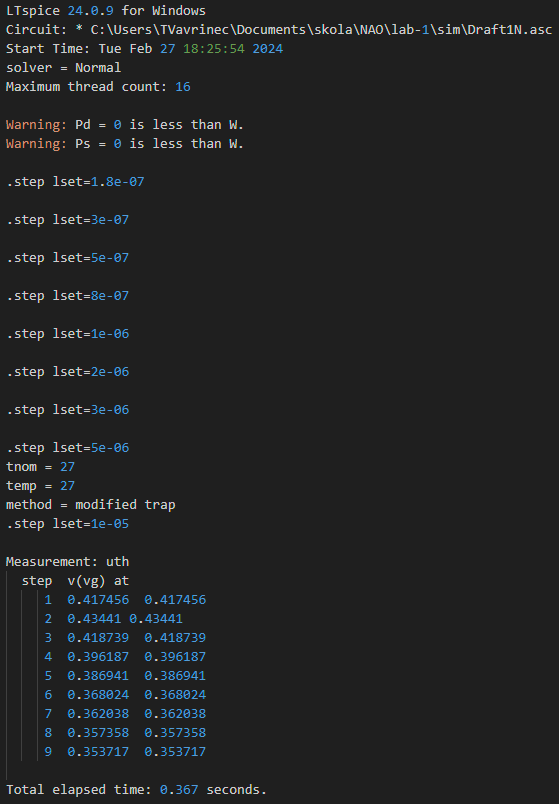
\includegraphics[height=0.4\textheight]{log/N-UTH0-WL_const.png}
        \centering{(NMOS)}
    \end{minipage}
    \hfill
    \begin{minipage}{0.5\textwidth}
        \centering
        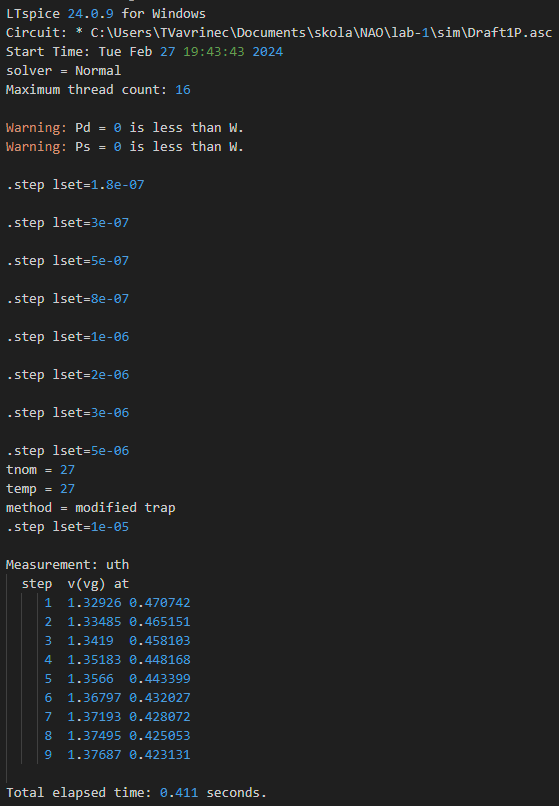
\includegraphics[height=0.4\textheight]{log/P-UTH0-WL_const.png}
        \centering{(PMOS)}
    \end{minipage}
    \caption{\label{fig:log_NP_WL_const} Printscreeny logů simulací při konstantním poměru \(W/L = 5\) pro NMOS i PMOS}
\end{figure}

\begin{table}[H]
    \begin{minipage}{0.5\textwidth}
        \centering
        \begin{tabular}{|c|c|}
            \hline
            \(L [\mu m]\) & \(U_{TH0} [V]\) \\ \hline
            0.18	      & 0.417456        \\ \hline
            0.3	          & 0.434410        \\ \hline
            0.5	          & 0.418739        \\ \hline
            0.8	          & 0.396187        \\ \hline
            1	          & 0.386941        \\ \hline
            2	          & 0.368024        \\ \hline
            3	          & 0.362038        \\ \hline
            5	          & 0.357358        \\ \hline
            10	          & 0.353717        \\ \hline
        \end{tabular}

        \vspace{5mm}
        \centering{(NMOS)}
    \end{minipage}
    \hfill
    \begin{minipage}{0.5\textwidth}
        \centering
        \begin{tabular}{|c|c|}
            \hline
            \(L [\mu m]\) & \(U_{TH0} [V]\) \\ \hline
            0.18          & 0.470742        \\ \hline
            0.3	          & 0.465151        \\ \hline
            0.5	          & 0.458103        \\ \hline
            0.8	          & 0.448168        \\ \hline
            1             & 0.443399        \\ \hline
            2  	          & 0.432027        \\ \hline
            3  	          & 0.428072        \\ \hline
            5  	          & 0.425053        \\ \hline
            10 	          & 0.423131        \\ \hline
        \end{tabular}

        \vspace{5mm}
        \centering{(PMOS)}
    \end{minipage}

    \caption{\label{tab:N_wl_const} Výsledky simulace při konstantním poměru \(W/L = 5\)}
\end{table}

\newpage
\subsubsection{Prahové napětí \(U_{TH0}\) při různém poměru \(W/L\)}
\begin{lstlisting}[language=Spice, caption={Použitý kod simulace při různém poměru \(W/L\)}]
.lib cmos018.txt
.param wset=table(n, 1,0.22u, 2,1u, 3,2u, 4,2u, 5,5u, 6,5u, 7,10u, 8,10u, 9,40u)
.param lset=table(n, 1,0.18u, 2,0.5u, 3,0.5u, 4,1u, 5,1u, 6,2u, 7,5u, 8,10u, 9,10u)
.step param n 1 9 1
.meas DC UTH FIND V(VG) WHEN Id(M1)=100n*wset/lset
.dc VGS2 0 1 1m
\end{lstlisting}

\begin{figure}[H]
    \begin{minipage}{0.5\textwidth}
        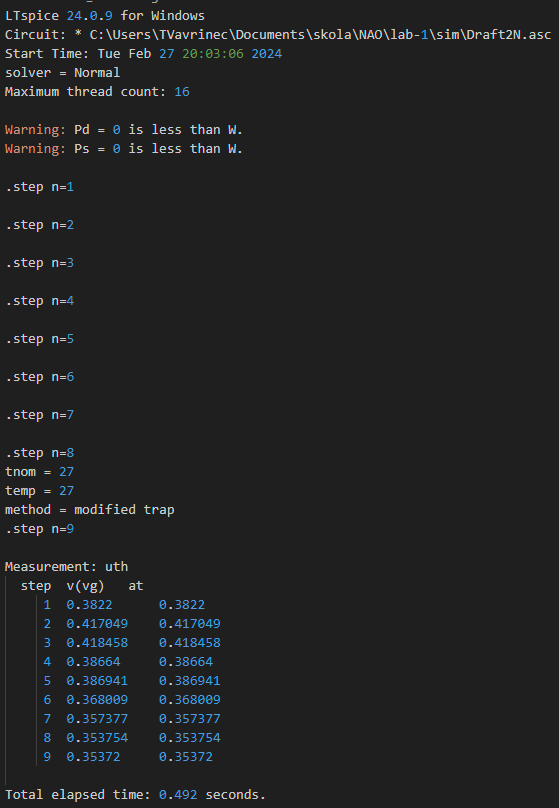
\includegraphics[height=0.4\textheight]{log/N-UTH00-WL_dinamic.png}
        \centering{(NMOS)}
    \end{minipage}
    \hfill
    \begin{minipage}{0.5\textwidth}
        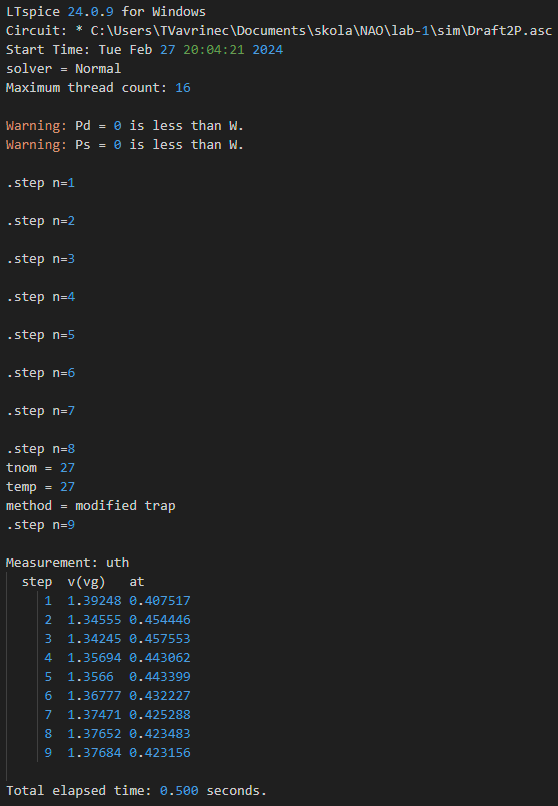
\includegraphics[height=0.4\textheight]{log/P-UTH00-WL_dinamic.png}
        \centering{(PMOS)}
    \end{minipage}
    \caption{\label{fig:log_NP_WL_const} Printscreeny logů simulací ruzných pomněru \(W/L\) pro NMOS i PMOS}
\end{figure}

\begin{table}[H]
    \begin{minipage}{0.5\textwidth}
        \centering
        \begin{tabular}{|c|c|c|}
            \hline
            \(L [\mu m]\) & \(W [\mu m]\) & \(U_{TH0} [V]\) \\ \hline
            0.22          & 0.18          & 0.382200        \\ \hline
            1	          & 0.5           & 0.417049	    \\ \hline
            2	          & 0.5           & 0.418458	    \\ \hline
            2	          & 1             & 0.386640        \\ \hline
            5             & 1             & 0.386941	    \\ \hline
            5  	          & 2             & 0.368009	    \\ \hline
            10 	          & 5             & 0.357377	    \\ \hline
            10 	          & 10            & 0.353754	    \\ \hline
            40 	          & 10            & 0.353720        \\ \hline
        \end{tabular}

        \vspace{5mm}
        \centering{(NMOS)}
    \end{minipage}
    \hfill
    \begin{minipage}{0.5\textwidth}
        \centering
        \begin{tabular}{|c|c|c|}
            \hline
            \(L [\mu m]\) & \(W [\mu m]\) & \(U_{TH0} [V]\) \\ \hline
            0.22          & 0.18          & 0.407517        \\ \hline
            1	          & 0.5           & 0.454446        \\ \hline
            2	          & 0.5           & 0.457553        \\ \hline
            2	          & 1             & 0.443062        \\ \hline
            5             & 1             & 0.443399        \\ \hline
            5  	          & 2             & 0.432227        \\ \hline
            10 	          & 5             & 0.425288        \\ \hline
            10 	          & 10            & 0.423483        \\ \hline
            40 	          & 10            & 0.423156        \\ \hline
        \end{tabular}

        \vspace{5mm}
        \centering{(PMOS)}
    \end{minipage}

    \caption{\label{tab:N_wl_const} Výsledky simulace při různém poměru \(W/L = 5\)}
\end{table}
